%!TEX root = ../main.tex
%%%%%%%%%%%%%%%%%%%%%%%%%%%%%%%%%%
% Links:
%
% Difficulty:
% Companies: 
%%%%%%%%%%%%%%%%%%%%%%%%%%%%%%%%%%

\chapter{Clone a linked list with random pointer}
\label{ch:clone_list_random_pointer}
\section*{Introduction}
This chapter discusses a very interesting problem on (an unconvential type of) linked lists.
The kind of linked list we are dealing with here is a singly linked, with an additional pointer that \textbf{might} point to another node in the list. 
The \CC definition of said list is given in Listing \ref{list:delete_duplicates_list:linked_list} where we can notice the additional field \inline{random} which differentiates it from the other more canonical linked list definitions seen in other chapters (see Chapter \ref{ch:delete_duplicates_list} and Listing \ref{list:delete_duplicates_list:linked_list}).

\begin{lstlisting}[language=c++, caption={Definition of a linked list with a pointer to a \textit{random} node.},label=list:delete_duplicates_list:linked_list]

template <class T> 
class Node
{
  public:
  T val{};
  Node *next{nullptr}; //points to the next element in the list
  Node *random{nullptr}; //nullptr or points to any other node in the list.

  Node(const T &_val)
  {
    val    = _val;
    next   = nullptr;
    random = nullptr;
  }
};
\end{lstlisting}

\section{Problem statement}
\begin{exercise}
Write a function that, given a linked list $L$ of the type defined in Listing \ref{list:clone_list_random_pointer:list_definition} returns a deep-copy of $L$.

In this chapter we will be graphically representing a list as a sequence of pairs of integers. A pair $(v,r)$ represent a node of the list where:
\begin{itemize}
	\item $v$ is the payload of the node
	\item $r$ is the index of the node that the random pointer points to. $-1$ represents \lstinline[columns=fixed]{nullptr}.
\end{itemize} 
For instance the sequence $[(7,-1),(13,0),(11,4),(10,2),(1,0)]$ represent the list shown in Figure \ref{fig:clone_list_random_pointer:list1}.
\end{exercise}

\begin{figure}
	\label{fig:clone_list_random_pointer:list1}
	\centering
	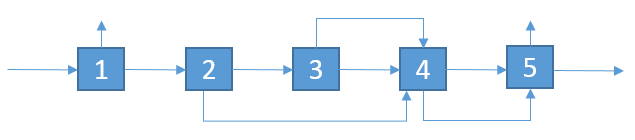
\includegraphics[scale=0.6]{sources/clone_list_random_pointer/images/random_list_1}
	\caption{Linked list wit random pointer. Each node has two outgoing arrows represening. One for the \textit{next} and the other for the \textit{random} node.}
\end{figure}


\section{Clarification Questions}
The problem is intended to test list manipulation skills and it is not really about complex algorithm design.
As such,  questions about the size of the input aimed at getting a feel for the type of time complexity expected does not help much.
Rather, it is better to ask questions relating to the structure of the list itself in order to identify any pattern in the list we could take advantage of.

\begin{QandA}
	\begin{questionitem} \begin{question} Is it guaranteed that at least one not-null random pointer exists?  \end{question} 	 
    \begin{answered}
		\textit{No, all random pointer might be null.}
	\end{answered} \end{questionitem}
	\begin{questionitem} \begin{question} Can a random pointer point to itself?  \end{question} 	 
    \begin{answered}
		\textit{Yes, you can have a node pointing to itself.}
	\end{answered} \end{questionitem}

	\begin{questionitem} \begin{question} Does the random pointer always point to a node ahead in the list?  \end{question} 	 
		\begin{answered}
			\textit{No, the random pointer can point to any node.}
		\end{answered} \end{questionitem}
	
\end{QandA}

\section{Discussion}
\label{clone_list_random_pointer:sec:discussion}

In the following section we are going to have a look at two solutions that are fundamentally different from each other in terms of time and space complexity.
The first of the two, the one in Section \ref{clone_list_random_pointer:sec:bruteforce}, uses additional memory (linear amount) while the second one (see Section \ref{clone_list_random_pointer:sec:interleaved_lists}) works in constant time but, at the cost of being more complex and significantly harder to come up with during an interview.

\subsection{Linear memory solution}
\label{clone_list_random_pointer:sec:bruteforce}
The core idea behind the solution presented in this section can be conceptually divided into $4$ steps:
\begin{enumerate}
	\item We start by creating as many empty nodes as in the original list. We save the pointers to these new nodes in a vector \inline{std::vector<Node<T>*> ptrs;}.
	\item In the next step we want to map the pointers to the nodes in the original list to their indices (the distance from the head node). 
	We can do this while traversing the list from head to tail. 
	We do this because we want to remember for each node its index  in the original list. 
	\item We can proceed now in fixing all the \inline{next} pointers of the nodes in \inline{ptrs} so that \lstinline[columns=fixed]{ptrs[i]->next} points to  \lstinline[columns=fixed]{ptrs[i+1]}. At this point we have a new singly linked list with broken random pointers. Basically an half-cloned list.
	\item We can traverse the original list once again, and if the current node $c$ has a not-null random pointer \inline{c->random} we can query the map we filled in step $2$ to know the index of the node \inline{c->random}. Once we have this information, we can fix the random pointer of the copy of $c$ in \inline{ptrs}.
\end{enumerate}
An implementation of this idea is shown in  Listing \ref{list:clone_list_random_pointer_1}


\lstinputlisting[language=c++, caption={Linear memory solution.},label=list:clone_list_random_pointer_1]{sources/clone_list_random_pointer/clone_list_random_pointer_solution1.cpp}

The first \inline{while} takes care of creating the copy nodes and to fill-up the maps $P$ containing the information about the index of a node.

The subsequence \inline{for} connects the \inline{next} pointers in the copy nodes and the final \inline{while} traverses the list from head to tail and takes care of fixing the copy nodes random pointers suing theinformation in the map $P$.

Listing \ref{list:clone_list_random_pointer_1}  has linear time and space  complexity. 
The time complexity is already optimal as we cannot do better than linear time considering that in order to create a copy we need to look at all the nodes at least once. The space complexity can be improved though, and as we will see in Section \ref{clone_list_random_pointer:sec:interleaved_lists},   can actually be brought down to constant.


\subsection{Constant memory solution}
\label{clone_list_random_pointer:sec:interleaved_lists}
The idea behind the solution presented in this section is to construct the copy such that its nodes are interleaved with the ones from the original list. We are going to embeed the copy inside the original list.
The solution in this section is divided into three steps where:
\begin{enumerate}
	\item we create an initial copy interleaved in the original list (see Section \ref{clone_list_random_pointer:sec:interleaved_lists1});
	\item then, the random pointers are fixed (see Section  \ref{clone_list_random_pointer:sec:interleaved_lists2});
	\item finally, the cloned list is extracted-out from the original list and returned (see Section  \ref{clone_list_random_pointer:sec:interleaved_lists3}).
\end{enumerate}

\subsubsection{Copy interleaved with the original list}
\label{clone_list_random_pointer:sec:interleaved_lists1}
This is the easiest of the three steps and it only requires to create a copy of a node at index $i$ and place it at index $i+1$. 
For instance given the input list\footnote{Remember that $(x,-1)$ is a node containing the value $x$ and with random pointer set to \lstinline[columns=fixed]{nullptr}}: $A = [(7,-1),(13,0),(11,4),(10,2),(1,0)]$ we want to have an interleaved list that look like the following: $A' = [(7,-1),(7,-1),(13,0),(13,-1),(11,4),,(11,-1),(10,2),(10,-1),(1,0),(1,0)]$ (see Figure \ref{fig:clone_list_random_pointer:interleaved}).
Every node at even indices is a copy of its predecessor except that it has the random pointer set to \lstinline[columns=fixed]{nullptr}.

This step is implemented in the function \lstinline[columns=fixed]{fix_random_pointers} in Listing \ref{list:clone_list_random_pointer_2}.

Given the original list is  $A= a_0 \rightarrow a_1 \rightarrow \ldots \rightarrow a{n-1}$ and the copy of a A is $B = b_0 \rightarrow b_1 \rightarrow \ldots \rightarrow b{n-1}$ what we achieved in this step a new list $I$ of size $2n$: $I=a_0 \rightarrow b_0 \rightarrow a_1 \rightarrow b_1 \rightarrow a_2 \rightarrow b_2 \rightarrow \ldots \rightarrow a_{n-1} \rightarrow b_{n-1}$.

\begin{figure}
	\centering
	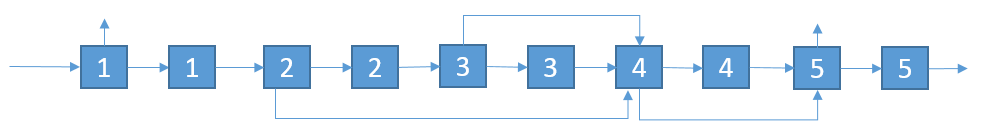
\includegraphics[scale=0.5]{sources/clone_list_random_pointer/images/random_list_2}
	\caption{Intermediate interleaved list.}
	\label{fig:clone_list_random_pointer:interleaved}
\end{figure}


\subsubsection{Fix the random pointers in the interleaved list}
\label{clone_list_random_pointer:sec:interleaved_lists2}
Having the two lists  $A$ (the original) and $B$ (the copied) arranged this way is quite useful because we can still visit the original lists and at the same time operate on its mirror by simply modifying the nodes at odd indexes.

An interleaved list always has an even number of nodes. 
All the ones at even positions $(0,2,\ldots)$ belong to the original lists while all the nodes with odd indexes $(1,3,\ldots)$ to the copy.
Given a node $n_{2k}=(x,r)$ at an even index $2k$, we can fix the random pointer for the copy of this node $n_{2k+1}=(x,-1)$ at index $2k+1$ by simply fixing its random pointer to the value pointed by $n_{2k}$\lstinline[columns=fixed]{->random->next}. See Figure \ref{fig:clone_list_random_pointer:interleaved_fixed} where the red lines represent the mirrored for the random pointers in the original list and function \lstinline[columns=fixed]{split_fix_random_pointers} in Listing \ref{list:clone_list_random_pointer_2}.

\begin{figure}
	\centering
	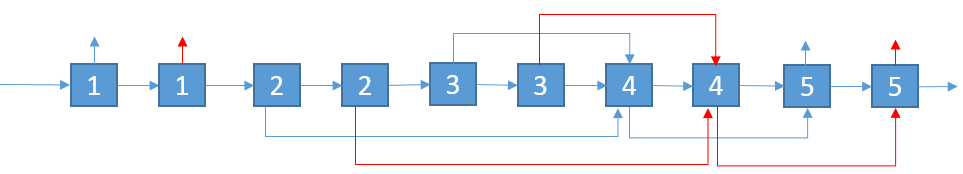
\includegraphics[scale=0.5]{sources/clone_list_random_pointer/images/random_list_3}
	\caption{Interleaved list with fixed random pointers.}
	\label{fig:clone_list_random_pointer:interleaved_fixed}
\end{figure}

\subsubsection{Extract the cloned list}
\label{clone_list_random_pointer:sec:interleaved_lists3}
Once we reach this point, we have basically two copies of the original list (with random pointers fixed) interleaved with each other. 
All it is necessary at this point is to pull out the cloned list. 
This is easily achievable as all we need to do is to remove all the odd nodes, and in the process stich the noded at even indices together.
This step is imnplemented in the function \lstinline[columns=fixed]{split_list} in Listing \ref{list:clone_list_random_pointer_2}).

The full implementation of this solution is shown in Listing  \ref{list:clone_list_random_pointer_2}.

\lstinputlisting[language=c++, caption={Constant memory solution.},label=list:clone_list_random_pointer_2]{sources/clone_list_random_pointer/clone_list_random_pointer_solution2.cpp}